%!TeX root=../pridetop.tex

\headlesschapter{Chapter \thechapter}

\begin{pictures}
\begin{a4}
	\begin{figure}[t!]
		\centering
		\captionlistentry{Headpiece to Chapter \thechapter}
		\begin{tikzpicture}[remember picture, overlay]  
			\node (img) at ($(current page.north)+(0cm,-10.5cm)$) {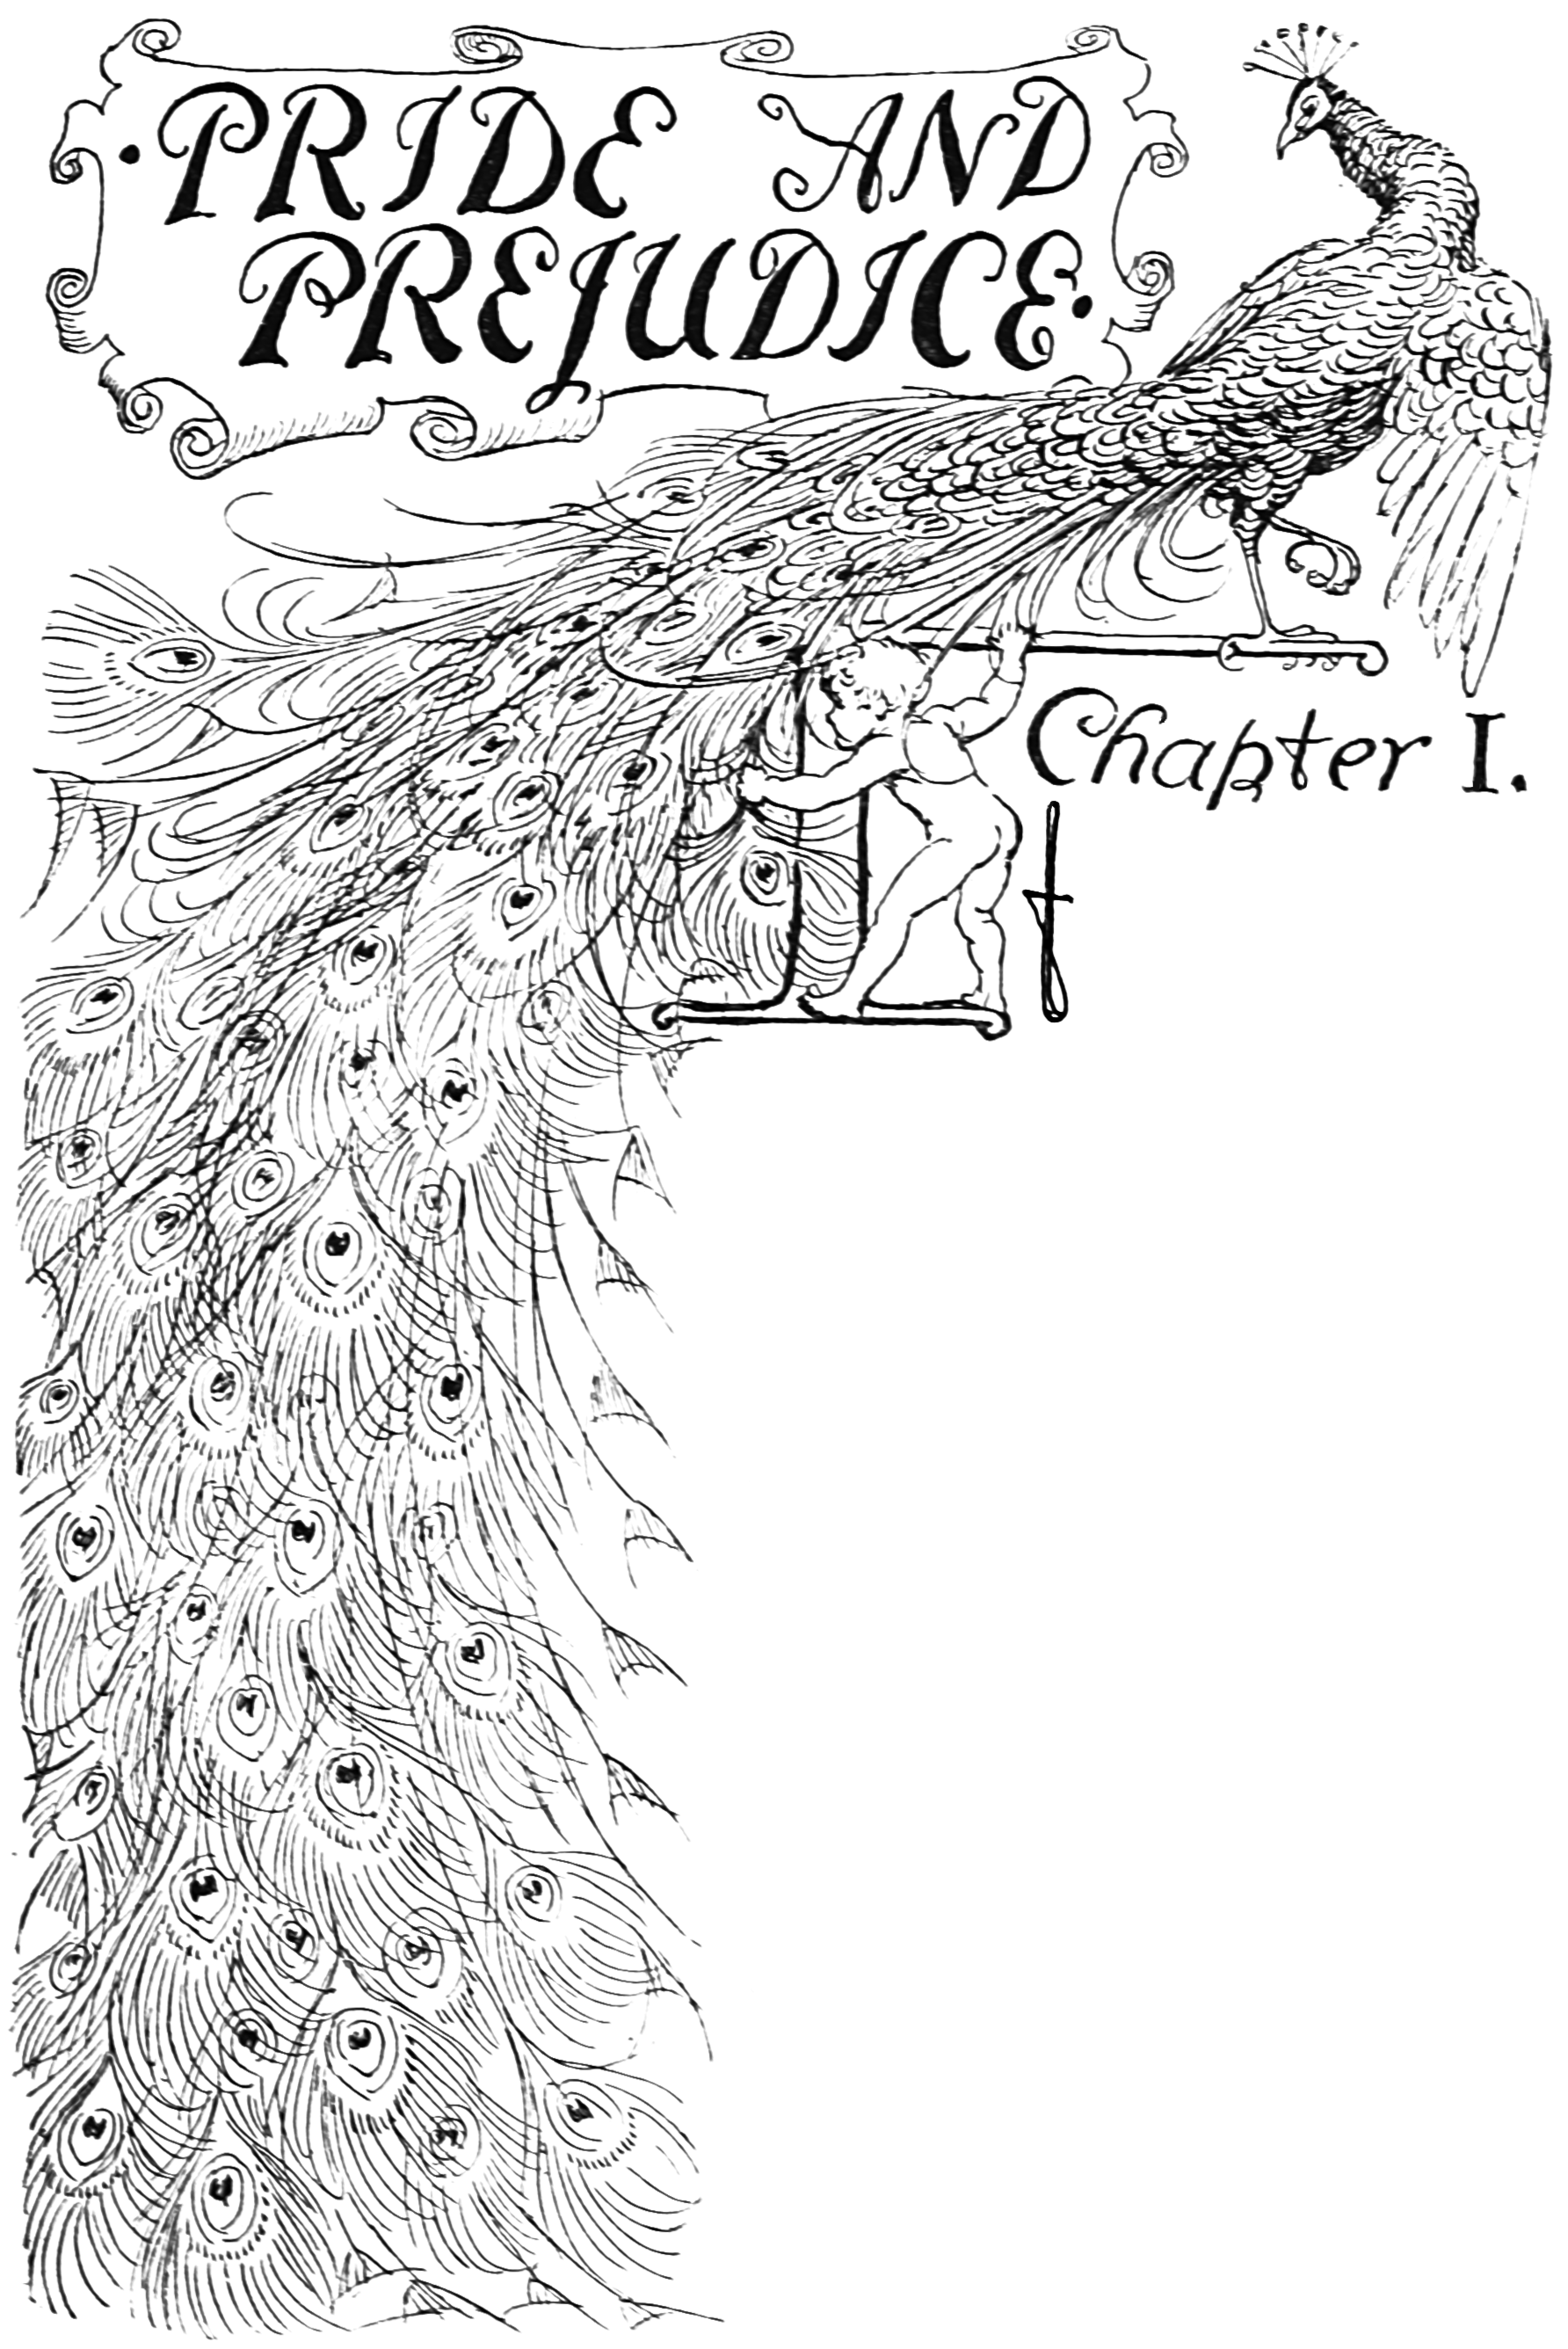
\includegraphics[width=1.15\linewidth]{1top}};
			\node[text width=0.26\textwidth, align=justify] (toptext) at (4.1,1.5) {is a truth universally acknowledged, that};
			\node[below=5.5cm of toptext.east, anchor=east, text width=0.48\textwidth,align=justify] (bottomtext) {
	a single man in possession of a good fortune must be in want of a wife. However little known the feelings or views of such a man may be on his first entering a neighbourhood, this truth is so well fixed in the minds of the surrounding families, that he is considered as the rightful property of some one or other of their daughters.
			\parindent=1em

			<My dear Mr Bennet,> said his lady to him one day, <have you heard that Netherfield Park is let at last?>

			Mr Bennet replied that he had not.

			<But it is,> returned she; <for Mrs Long has just been here, and she told me all about it.>

			Mr Bennet made no answer.

			<Do not you want to know who has taken it?> cried his wife, impatiently.

			<You want to tell me, and I have no objection to hearing it.>
			};
		\end{tikzpicture}
	\end{figure}
\end{a4}

\begin{letter}
	 
	\begin{figure}[t!]
		\centering
		\captionlistentry{Headpiece to Chapter \thechapter}
		\begin{tikzpicture}[remember picture, overlay]
	  
			\node (img) at ($(current page.north)+(0cm,-10.5cm)$) {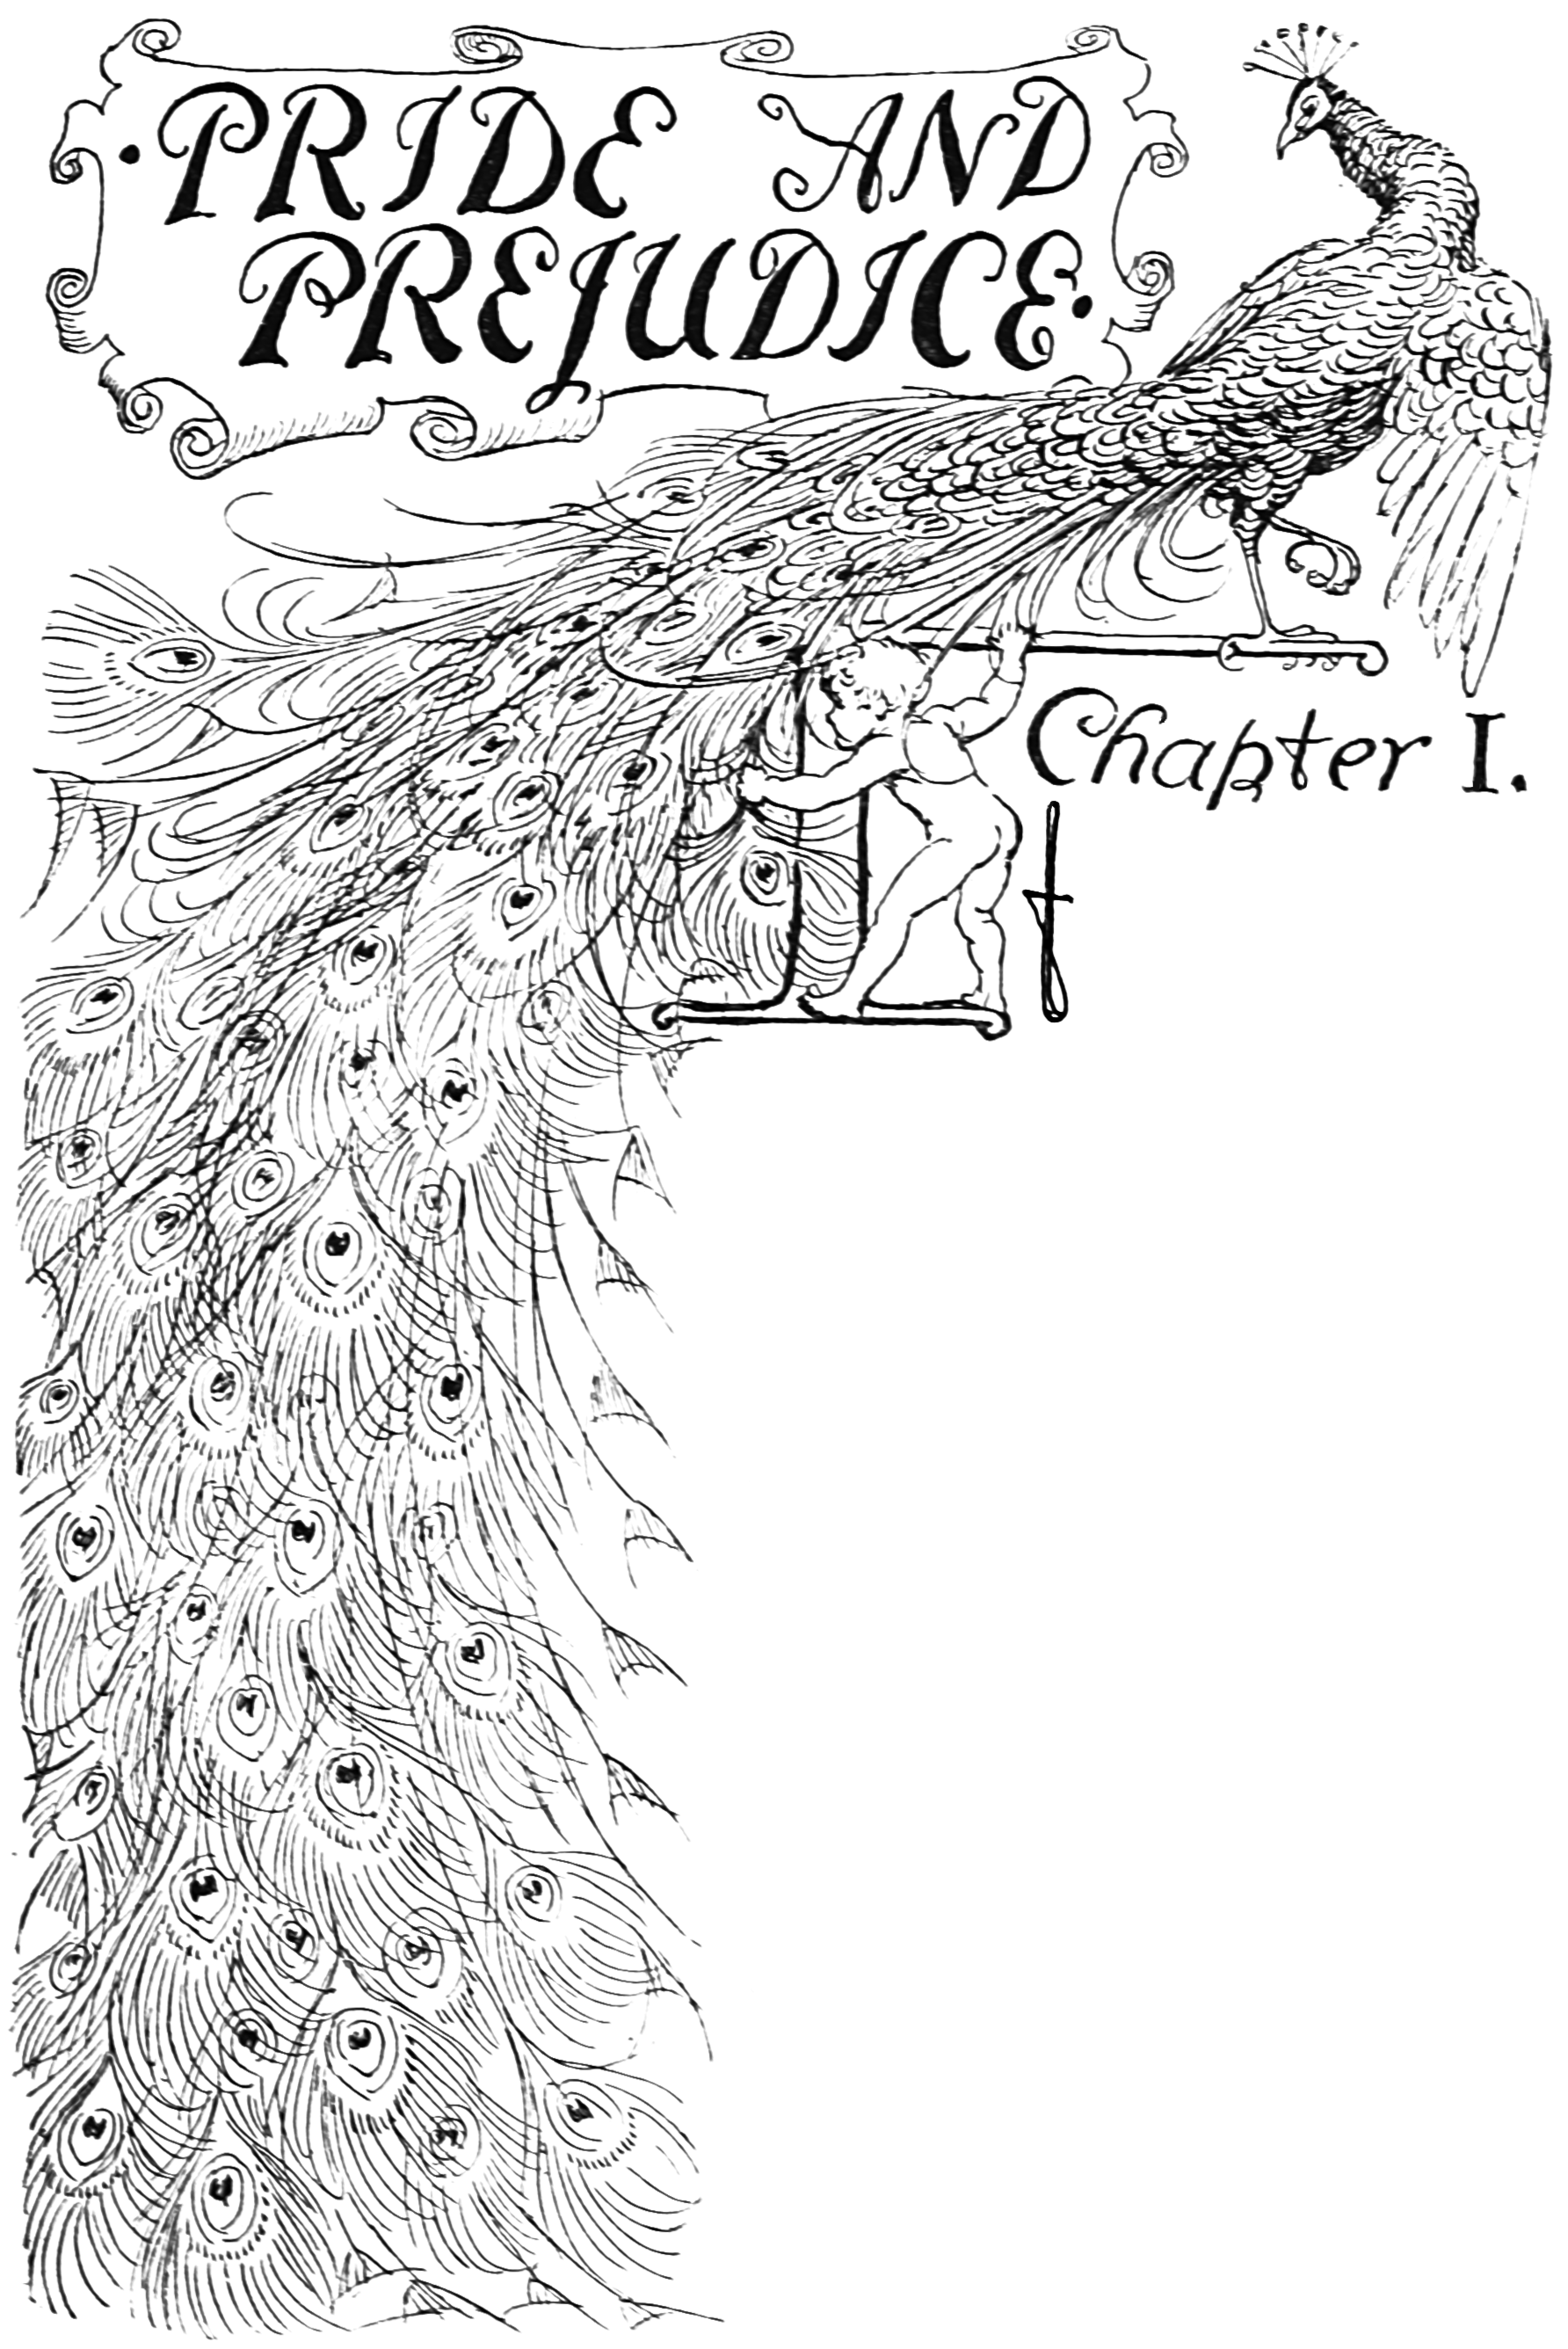
\includegraphics[width=1.2\linewidth]{1top}};
			\node[text width=0.3\textwidth, align=justify] (toptext) at (4.2,1.8) {is a truth universally acknowledged, that a};
			\node[below=5.52cm of toptext.east, anchor=east, text width=0.55\textwidth,align=justify] (bottomtext) {
	single man in possession of a good fortune must be in want of a wife. However little known the feelings or views of such a man may be on his first entering a neighbourhood, this truth is so well fixed in the minds of the surrounding families, that he is considered as the rightful property of some one or other of their daughters.
			\parindent=1em

			<My dear Mr Bennet,> said his lady to him one day, <have you heard that Netherfield Park is let at last?>

			Mr Bennet replied that he had not.

			<But it is,> returned she; <for Mrs Long has just been here, and she told me all about it.>

			Mr Bennet made no answer.

			<Do not you want to know who has taken it?> cried his wife, impatiently.

			<You want to tell me, and I have no objection to hearing it.>
			};
		\end{tikzpicture}
	\end{figure}
%	\enlargethispage{3cm}
\end{letter}

 \thispagestyle{plain}
 \clearpage
\end{pictures}

\begin{placeholder}
It is a truth universally acknowledged, that a single man in possession of a good fortune must be in want of a wife. However little known the feelings or views of such a man may be on his first entering a neighbourhood, this truth is so well fixed in the minds of the surrounding families, that he is considered as the rightful property of some one or other of their daughters.

<My dear Mr Bennet,> said his lady to him one day, <have you heard that Netherfield Park is let at last?>

Mr Bennet replied that he had not.

<But it is,> returned she; <for Mrs Long has just been here, and she told me all about it.>

Mr Bennet made no answer.
<Do not you want to know who has taken it?> cried his wife, impatiently.

<You want to tell me, and I have no objection to hearing it.>
\clearpage
\end{placeholder}

This was invitation enough.

<Why, my dear, you must know, Mrs Long says that Netherfield is taken by a young man of large fortune from the north of England; that he came down on Monday in a chaise and four to see the place, and was so much delighted with it that he agreed with Mr Morris immediately; that he is to take possession before Michaelmas, and some of his servants are to be in the house by the end of next week.>

\begin{figure}[tbh]
\centering
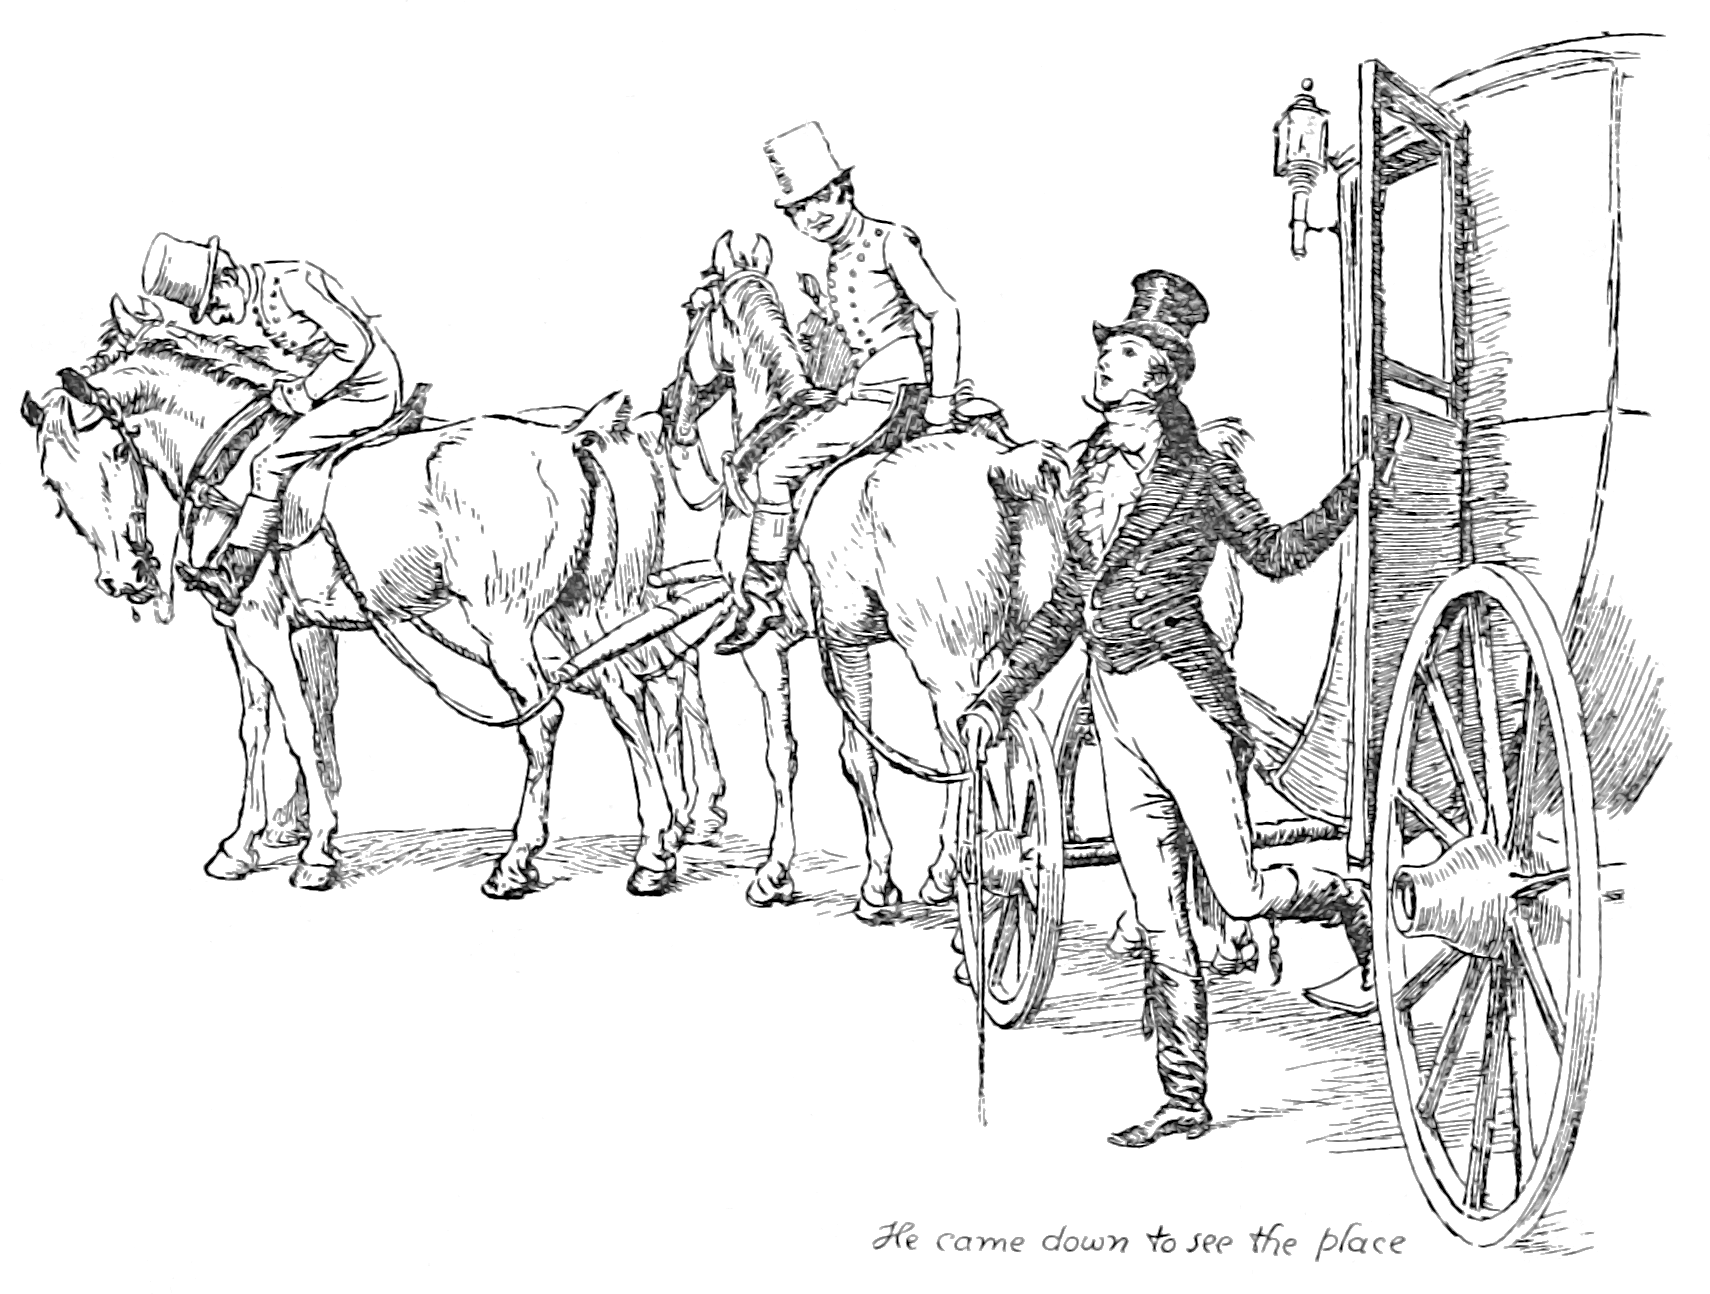
\includegraphics[width=\linewidth]{1camedown}
\captionlistentry{He came down to see the place}
\end{figure}

<What is his name?>

<Bingley.>

<Is he married or single?>

<Oh, single, my dear, to be sure! A single man of large fortune; four or five thousand a year. What a fine thing for our girls!>

<How so? how can it affect them?>

<My dear Mr Bennet,> replied his wife, <how can you be so tiresome? You must know that I am thinking of his marrying one of them.>

<Is that his design in settling here?>

<Design? Nonsense, how can you talk so! But it is very likely that he \textit{may} fall in love with one of them, and therefore you must visit him as soon as he comes.>

<I see no occasion for that. You and the girls may go—or you may send them by themselves, which perhaps will be still better; for as you are as handsome as any of them, Mr Bingley might like you the best of the party.>

<My dear, you flatter me. I certainly \textit{have} had my share of beauty, but I do not pretend to be anything extraordinary now. When a woman has five grown-up daughters, she ought to give over thinking of her own beauty.>

<In such cases, a woman has not often much beauty to think of.>

<But, my dear, you must indeed go and see Mr Bingley when he comes into the neighbourhood.>

<It is more than I engage for, I assure you.>

<But consider your daughters. Only think what an establishment it would be for one of them. Sir William and Lady Lucas are determined to go, merely on that account; for in general, you know, they visit no new comers. Indeed you must go, for it will be impossible for \textit{us} to visit him, if you do not.>

<You are over scrupulous, surely. I dare say Mr Bingley will be very glad to see you; and I will send a few lines by you to assure him of my hearty consent to his marrying whichever he chooses of the girls—though I must throw in a good word for my little Lizzy.>

\begin{figure}[bh!]
\centering
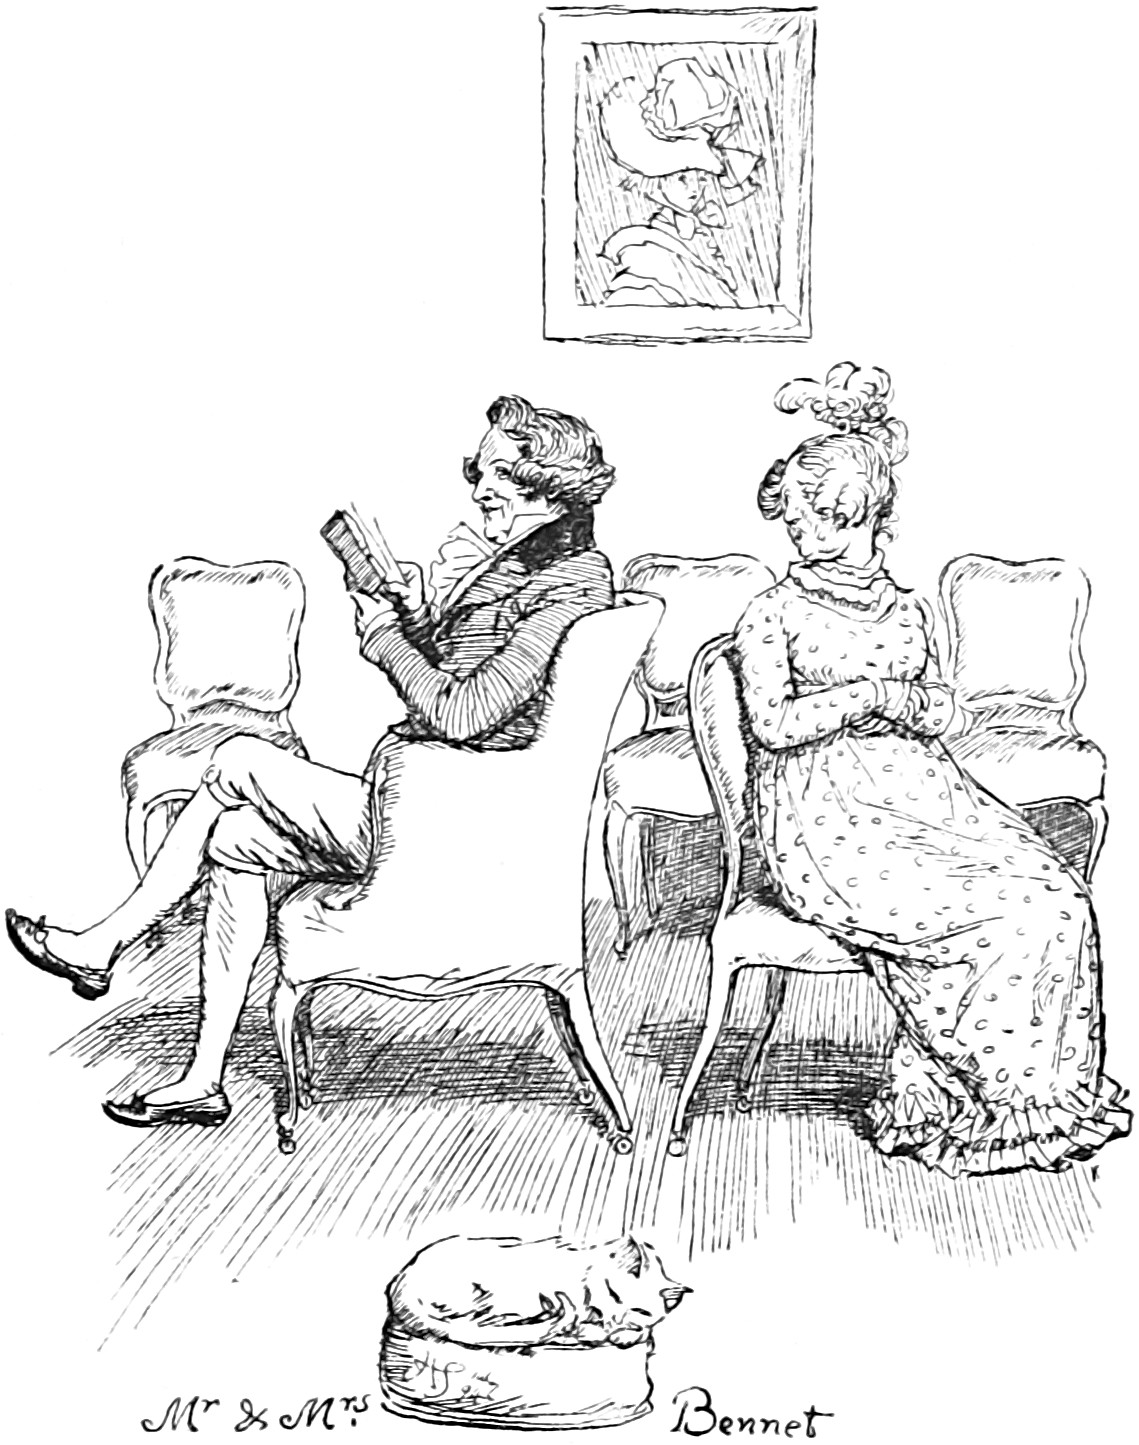
\includegraphics[width=.8\linewidth]{1mrmrs}
\captionlistentry{Mr \& Mrs Bennet}
\end{figure}

<I desire you will do no such thing. Lizzy is not a bit better than the others: and I am sure she is not half so handsome as Jane, nor half so good-humoured as Lydia. But you are always giving \textit{her} the preference.>

<They have none of them much to recommend them,> replied he: <they are all silly and ignorant like other girls; but Lizzy has something more of quickness than her sisters.>

<Mr Bennet, how can you abuse your own children in such a way? You take delight in vexing me. You have no compassion on my poor nerves.>

<You mistake me, my dear. I have a high respect for your nerves. They are my old friends. I have heard you mention them with consideration these twenty years at least.>

<Ah, you do not know what I suffer.>

<But I hope you will get over it, and live to see many young men of four thousand a year come into the neighbourhood.>

<It will be no use to us, if twenty such should come, since you will not visit them.>

<Depend upon it, my dear, that when there are twenty, I will visit them all.>

Mr Bennet was so odd a mixture of quick parts, sarcastic humour, reserve, and caprice, that the experience of three-and-twenty years had been insufficient to make his wife understand his character. \textit{Her} mind was less difficult to develope. She was a woman of mean understanding, little information, and uncertain temper. When she was discontented, she fancied herself nervous. The business of her life was to get her daughters married: its solace was visiting and news.

